\section{Theory}
Electron Spin Resonance (ESR) is a spectroscopic method employed to identify unpaired electrons in substances such as free radicals or transition metals. By applying a magnetic field and electromagnetic radiation (in the microwave or radio wave range), ESR measures transitions between electron spin states, providing insights into the local electronic and magnetic environment. ESR is widely utilized in chemistry, physics, biology, and materials science for investigating molecular structure, magnetic properties, and defects in materials.

The fundamentals of elementary magnetic resonance may be understood in terms of simple classical concepts. When a magnetic moment is placed in external magnetic field it experiences a torque Then the moment $\mu$ precess around magnetic field $H_0$ with
and angular Lamor frequency given by,

\begin{align}
    \omega_0 = g\left(\frac{e}{2mc}\right)H_0
\end{align}

where $g$ is Lande's g-factor ($g=1$ for pure orbital
momentum and $g=2$ for a free electron spin). For
the case of anion in a crystal, the behaviour is
modified by the environment and the g- factor may
differ from the Lande's g-factor.
This effective g-factor is known as the spectroscopic splitting factor.
We now introduce an additional weak magnetic
field that lies in the xy-plane and rotates around
the z-axis in the same direction as the Larmor
precession, with an angular frequency $\omega_1$.
If $\omega_1$
differs from $\omega_0$, the angle between the field $H_1$ and
the magnetic moment $\mu$ will continuously change,
causing their interaction to average out to zero.
However, if $\omega_1=\omega_0$, the angle between $\mu$ and
$H_1$ remains constant, resulting in an effective net
interaction.

When viewed in a reference frame rotating around
the z-axis with angular velocity $\omega_0$, the spin appears
to make an angle $\phi = 90◦ - \theta$ with $H_1$, and as
a result, begins to precess (in the rotating frame)
around $H_1$. This behavior is referred to as \textit{nutation} leading to a change in the angle $\theta$, which implies a change in the particle's potential energy in the
magnetic field. The change in $\theta$ is the classical analogy of a transition between sublevels with different
magnetic quantum numbers $m$. Such transitions can
only occur if the rotating field's angular frequency
$\omega_1=\omega_0$.

\begin{figure}[H]
    \centering
    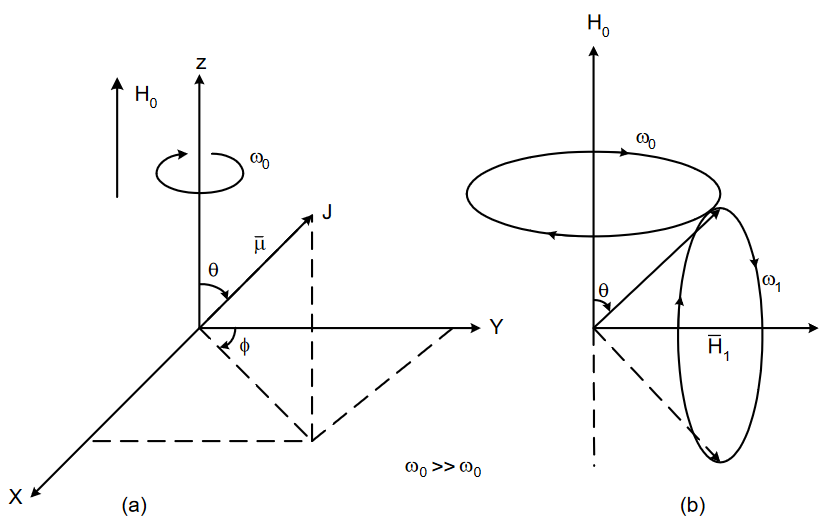
\includegraphics[width=1\columnwidth]{images/f1.png}
    \caption{Precession of magnetic moment $\mu$ when
    placed in magnetic field $H_1$ (a) Precession of the magnetic moment with frequency $\omega_0$ when no external
    magnetic field is applied, $\theta$ is constant (b) Precession
    of magnetic moment $\mu$ at a frequency $\omega_1$ when $H_1$ is
    applied, $\theta$ is not constant anymore.}
    \label{f1}
\end{figure}

\subsection*{Quantum Mechanical Picture}

Now, let's consider the quantum perspective of elementary magnetic resonance. Suppose the intrinsic
angular momentum of the electron, $S$, couples with
the orbital angular momentum, $L$, resulting in a total angular momentum $J$. The $J + 1$ magnetic sub-levels, labeled by the magnetic field $H_0$, have equal
energy differences between adjacent sublevels given
by

\begin{align}
    \Delta E = g\mu_B H_0
\end{align}

where $\mu_B$ is the Bohr magneton and $g$ is the Lande factor (or g-factor), whose correct quantum mechanical
value is

\begin{align}
    g = 1 + \frac{J(J+1)+S(S+1)-L(L+1)}{2J(J+1)}
\end{align}

If an alternating magnetic field perturbs the particle
with a frequency $\nu$, such that the quantum energy
$h\nu_1$ exactly matches the energy difference $\Delta E$ between the levels, and if the direction of the alternating field is perpendicular to the static magnetic field,
transitions will be induced between neighboring sub-levels according to the selection rule $\Delta m = \pm 1$ for
magnetic dipole radiation. The condition for resonance is,

\begin{align}
    \Delta E = g\mu_B H_0 = h\nu_0 = h\nu_1
\end{align}
Here, $\nu_1$ is the resonance frequency in cycles per second, which is identical to the classical condition $\omega_0=\omega_1$.

In atomic spectroscopy, transitions between sub-levels with different $m$ (labeled by $m$ with selection
rules $\Delta Lm = \pm 1$) are not directly observed. Instead,
the splitting of a level is detected as a small change
in the frequency of radiation emitted during transitions between widely separated energy levels. If we
could directly measure the frequency corresponding
to transitions between sublevels of the same state,
we would gain much more precise information about
the energy splitting.

\subsection*{Electron Paramagnetic Resonance\\and Spectroscopy}

Paramagnetic resonance is a crucial aspect of spectroscopy, offering a way to determine the energy levels of magnetic particles. It has unique characteristics that distinguish it from optical spectroscopy:\\

\begin{itemize}
    \item \textbf{Frequency Range:} Magnetic resonance experiments use frequencies ranging from $10^9$ to
    $10^{11}$ cycles per second. These frequencies,
    located below the infrared part of the spectrum,
    allow for highly precise investigation of small energy level splittings that are otherwise inaccessible or nearly inaccessible by optical methods.\\
    \item \textbf{Transition Probability:} The probability of
    spontaneous transitions in the radio-frequency
    range is very low, as it is proportional to $\nu^3$.
    Therefore, paramagnetic resonance studies rely
    solely on induced absorption and emission.\\
    \item \textbf{Transition Type:} While optical spectra
    typically result from electric dipole transitions
    between energy levels, paramagnetic resonance
    absorption lines arise exclusively from magnetic
    dipole transitions. Consequently, the Einstein
    coefficients for induced absorption and emission
    in paramagnetic resonance are smaller by approximately four orders of magnitude compared
    to optical transitions.\\
    \item \textbf{Detection Sensitivity:} The effect of paramagnetic resonance is extremely small. Its observation is possible due to the high sensitivity of
    electronic detection methods and the vast number of photons involved (1 mW corresponds to
    about $\approx 10^{20}$ photons per second at a frequency
    of $10^{10}$ cps).\\
    \item \textbf{Line Width:} In the optical frequency range, the line width is generally much smaller than fundamental frequency. However, in paramagnetic resonance, interactions that broaden the    
    lines can be of the same magnitude as the energy splitting that determines the resonance frequency. As a result, the width of paramagnetic
    resonance lines is often comparable to the fundamental frequency and can be measured with
    high precision. This allows for a detailed investigation of various interactions in paramagnetic
    substances by analyzing the shape and width
    of the paramagnetic resonance line and how it
    depends on different factors.\\
    \item \textbf{Monochromatic Radiation:} Unlike optical
    experiments, radio-frequency spectroscopy typically uses radiation that is so monochromatic
    that the generated frequency band is much narrower than the absorption line width.\\
    \item \textbf{Line Broadening Factors:} The key factors
    influencing line width include magnetic dipole
    interactions, exchange forces, local electric fields
    created by nearby magnetic particles, and thermal motion. The natural line widths of radio frequency spectra are negligible.\\
    \item \textbf{Spectral Study Method:} In paramagnetic
    resonance, spectra are not studied by varying
    the frequency of the incident radiation but by
    altering the characteristic frequencies of the absorbing systems. This is done by varying the
    static magnetic field.
\end{itemize}

In this experiment we are using Helmhlotz coil to
generate alternating magnetic field and Radio Frequency (RF) signal is provided to the sample.

\begin{figure}
    \centering
    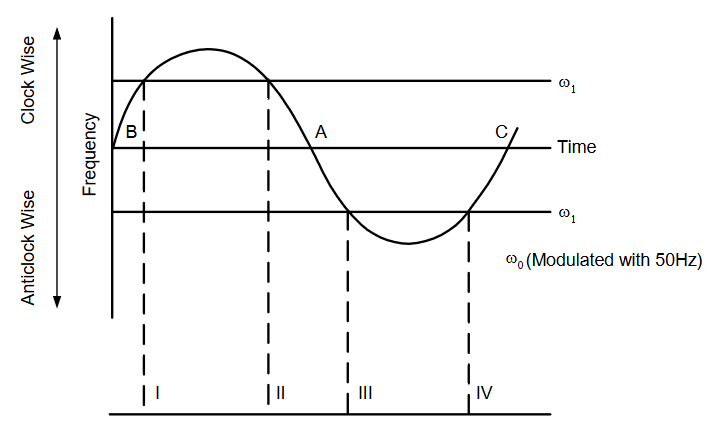
\includegraphics[width=0.7\columnwidth]{images/f3.png}
    \caption{The radio frequency is linear by polarised,
    which can be regarded as two circularly polarised
    fields of opposite direction (say clockwise and anti-
    clockwise). Further magnetic field $H_0$ also changes
    direction. Thus resonance occurs when the two frequencies ($\omega_1$ and $\omega_0$) becomes equal in magnitude as
    well as direction i.e. four times in one full cycle of
    $H_0$.}
    \label{f2}
\end{figure}

The observed peaks appear as absorption dips because the sample absorbs power from the induction
coil. These peaks result from the presence of an odd
number of inverting amplification stages in the circuit. The electron spin precesses at the Larmor frequency $\omega = eH_0/2mc$ and this frequency varies in both
magnitude and direction due to the alternating magnetic field $H_0$ generated by the Helmholtz coils. Resonance occurs when the radio frequency field $\omega_1$ falls
within the range of $\omega_0$, The positions of the four
peaks can be understood by referring to Fig. \ref{f2}. If
the X plate signal (50 Hz) and the Y plate signal
(ESR output) are in phase, then peaks I and II, as
well as peaks III and IV, will align. When $\omega_1 = \omega_0$
both in magnitude and direction, the peaks are seen. Here we
see that this happens 4 times in a full cycle of $H_0$.
We are able to witness EPR since DPPH is a paramagnetic compound and thus have a net non zero
magnetization. The magnetic field due to Helmholtz
coil is gven by

\begin{align}
    H = \frac{8\mu_0 N}{\sqrt{125} a}I
\end{align}

where $a$ is the radius of the coil and $N$ is the number
of turns. The peak to peak value of magnetic field is
$H_{pp} = 2\sqrt{2}H$. And the relation between the $H_0$ and
$H_{pp}$ is given by

\begin{align}
    H_0 = H_{pp}\frac{Q}{P}
\end{align}

Thus if we plot a graph between $1/Q$ and $H_{pp}$ the
slope is $1/(H_0 P)$.
% ============================================================================
\section{Experimental Setup}

\subsection*{Apparatus}
\begin{figure}[H]
    \centering
    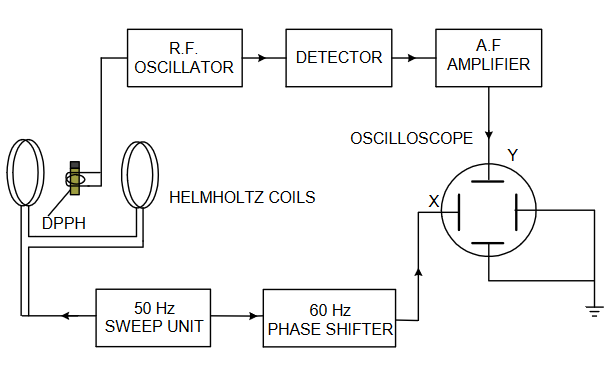
\includegraphics[width=1\columnwidth]{images/f2.png}
    \caption{Block Set Diagram of ESR}
    \label{f3}
\end{figure}
\begin{enumerate}
    \item ESR Spectrometer
    \item AC Gauss meter
    \item Cathode Ray oscilloscope
    \item Helmholtz Coil
    \item Paramagnetic substance (DPPH)\\
\end{enumerate}



The number of turns in each coil of Helmholtz coil
is 500 and the coils have a radius of 15.4 cm. The
separation between the two coils is 7.7cm.
A test sample, Diphenyl Picryl Hydrazyl (DPPH)
is placed in a plastic tube, which itself is in the
induction coils. This increases the filling factor to
the maximum. DPPH is a free radical and widely
used as a standard for ESR measurements.

\begin{figure}[H]
    \centering
    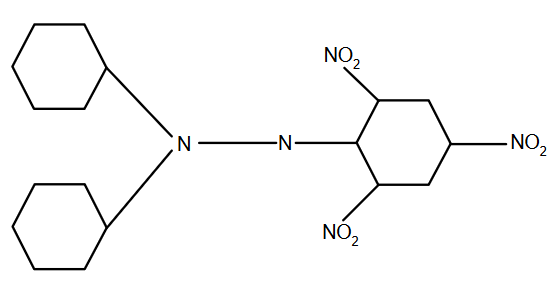
\includegraphics[width=.6\columnwidth]{images/f4.png}
    \caption{Chemical structure of DPPH}
\end{figure}